%==========================================================================
\chapter{Introduction}
%==========================================================================
In order to demonstrate that developing highly secure systems to the
level of rigour required by the higher assurance levels of the Common
Criteria is possible, the NSA has asked Praxis High Integrity Systems to
undertake a research project to re-develop part of an existing secure
system (the Tokeneer System) in accordance with their high-integrity
development process. This re-development work will then be used to
show the security community that is is possible to develop secure
systems rigorously in a cost effective manner.

This document is the formal specification, written using the Z
notation. This document specifies the behaviour of the core of the Token
ID Station (TIS) that is being re-developed.
It documents the second step in the Praxis high
integrity systems development approach. The whole process consists of:

\begin{enumerate}
\item
Requirements Analysis (the REVEAL process)
\item
{\bf Formal Specification (using the formal notation Z)}
\item
Design (the INFORMED process)
\item
Implementation in SPARK Ada
\item
Verification (using the SPARK Examiner toolset).
\end{enumerate}

%--------------------------------------------------------------------------
\section{Structure of this Specification}
%--------------------------------------------------------------------------
This specification is a formal model of the TIS core function
presented using the Z notation. 
The specification models TIS as a number of state components and a number of
operations that change the state.  The operations presented in this
specification cover:
\begin{itemize}
\item
user authentication and entry into the enclave;
\item
enrolment of TIS;
\item
administrator logon/logoff;
\item
archiving the log;
\item
updating of configuration data;
\item
shutdown;
\item
overriding the enclave door.
\end{itemize}
This specification specifically does not model user exit from the
enclave; there could also be further administrative operations above
and beyond those presented in this specification but
these are not considered. It is intended that the structure of the
specification should not preclude the addition of further administrative
operations. 

The specification is structured by presenting type constructs useful in the
modelling of TIS in the remainder of this section. 

Section \ref{sec:TIS} introduces the state that defines the TIS.
 
Section \ref{sec:Interfaces} covers accepting data
from the real world and updating the real world. 

Section \ref{sec:Internal} presents a number of partial operations on parts of
the TIS state, these are later used in the construction of the TIS
system operations. 

Section \ref{sec:UserEntry} presents the multi-phase user authentication and
entry operation.

Section \ref{sec:Enclave} describes all the system operations that
take place within the enclave. These are administrative operations.

Section \ref{sec:Start} defines the initial system and the state of TIS at
start-up.

Section \ref{sec:Whole} describes how the whole TIS core
works. Here we pull together the operations described through the remainder
of the specification.

Appendix \ref{chap:readZ} gives a brief introduction to reading Z. 

Appendix \ref{sec:Summary} discusses a number of issues that were raised during the
production of this specification.

Appendix \ref{sec:Pre} gives an informal justification of the
precondition of the whole operation by considering the preconditions
of its constituent parts.

Appendix \ref{sec:SRSTrace} provides a commentary on the tracing of
this document to the SRS \cite{SRS}. It also lists those requirements
from the SRS that do not
trace to the body of this specification. These are categorised by the
reason for exclusion.

Appendix \ref{sec:STTrace} provides a commentary on the tracing of
this document to the Security Target \cite{ST}. 

%--------------------------------------------------------------------------
\section{Trace units}
%--------------------------------------------------------------------------
\label{sec:Traceunit}
Each section of the specification has been tagged with a named {\em
traceunit} which will be used as a reference from later design
documents. All trace units in this document have the prefix ``FS''
identifying them as originating in the Formal Specification.

Most traceunits contain a list of requirements that are relevent to
that part of the specification. These are taken from the SRS
\cite{SRS} and Security Target \cite{ST}. 

For example consider the traceunit on page \pageref{page:firstTraceunit}. Here
the section on tokens is identified by the name {\em FS.Types.Tokens}
and this section is relevant to the satisfaction of a number of
requirements from the Protection Profile \cite{PP} including {\it
FCO\_NRO.2.1}.  
%--------------------------------------------------------------------------
\section{Z basics}
%--------------------------------------------------------------------------
This formal specification is written using the Z formal notation. \cite{Spivey}

%..............................
\subsection{Z comments}
%.............................
The intention is that someone unfamiliar with Z should be able to read this
specification and gain a complete understanding of the functionality
of the TIS system specified within.

We have attempted to make the informal commentary as complete and
unambiuous as possible. We have also separated out the parts of the
commentary that are only relevant for understanding the formal model,
as below:
\begin{Zcomment}
\item
Readers who are not interested in the formal model can skip these
sections of the commentary.
\end{Zcomment}

%...............................
\subsection{Reading Z}
%..............................
Readers of this specification are encouraged to read the Z formal notation. 
Reading the Z in the context of the commentary should disambiguate the
English. 

In Appendix \ref{chap:readZ} we explain the basics of how to read Z. 
These basic ideas should be sufficient to aid reading this
specification. For a more detailed description of the Z notation refer
to \cite{Spivey}.

%....................................
\subsection{Defining Optional Items}
%....................................

In order to be able to define optional items we make the following definitions.

\def\Nil{nil}%
\def\Optional{\mathop{\rm optional}}
\def\The{the~}%

%%pregen \Optional
\begin{zed}
        \Optional X == \{ x : \finset X | \# x \leq 1\}
\\      \Nil[X] == \emptyset[X]
\\      \The[X] == \{~x : X @ \{ x \} \mapsto x \}
\end{zed}

%--------------------------------------------------------------------------
\section{TIS Basic Types}
%--------------------------------------------------------------------------

\begin{traceunit}{FS.Types.Time}
\end{traceunit}

Time and date is some universal clock,
which for our purposes can be modelled as just the naturals.
\begin{zed}
	TIME == \nat
\end{zed}

We define a constant $zeroTime$ used at system initialisation.

\begin{zed}
        zeroTime == 0
\end{zed}

\begin{traceunit}{FS.Types.Presence}
\end{traceunit}

Many entities such as tokens, fingers and floppy disks may be
presented to the system and removed by the user. We monitor the
presence of these entities.
\begin{zed}
	PRESENCE ::= present | absent
\end{zed}

\begin{traceunit}{FS.Types.Clearance}
\end{traceunit}


$CLASS$ is the ordered classifications on document, areas, and people.
\begin{syntax}
	CLASS ::= & unmarked | unclassified | restricted | confidential |
		secret | topsecret
\end{syntax}

There may be other aspects to classification but these are not
modelled here.

\begin{schema}{Clearance}
	class: CLASS
\end{schema}

There is an ordering on the type $Clearance$. The function
$minClearance$  gives the minimum of a
pair of elements of type $Clearance$. This will be the Clearance with
the lowest class. The ordering on class is formally defined within the
design, informally $unmarked$ is the lowest class and $topsecret$ is
the highest class. 

\begin{axdef}
        minClearance : Clearance \cross Clearance \fun Clearance
\end{axdef}

\begin{traceunit}{FS.Types.Privilege}
\end{traceunit}


$PRIVILEGE$ is the role held by the Token user. This will determine
the privileges that the Token user has when interacting with the ID
station.
\begin{syntax}
        PRIVILEGE ::= & userOnly | guard | securityOfficer | auditManager 
\end{syntax}

\begin{traceunit}{FS.Types.User}
\end{traceunit}


A $USER$ is a unique identification of a certificate owner. For the
purpose of this specification it is a given type. 
 
\begin{zed}
	[ USER ]
\end{zed}

\begin{traceunit}{FS.Types.Issuer}
\end{traceunit}


An $ISSUER$ is a unique identification of an issuing body. Issuers are
privileged users with the ability to issue certificates. 
 
\begin{axdef}
ISSUER : \power USER
\end{axdef}

\begin{traceunit}{FS.Types.Fingerprint}
\end{traceunit}


$FINGERPRINT$ will need to include sufficient control information to allow
us to compare with templates and decide a match or not.
\begin{zed}
	[ FINGERPRINT ]
\end{zed}

\begin{traceunit}{FS.Types.FingerprintTemplate}
\end{traceunit}


A $FINGERPRINTTEMPLATE$ contains abstracted information, derived from
a number of sample readings of a fingerprint.

\begin{zed}
	[ FINGERPRINTTEMPLATE ]
\end{zed}

The fingerprint template and will be accompanied by additional information,
such as the threshold level to be applied to any comparisons.
This is not currently modelled.
\begin{schema}{FingerprintTemplate}
	template: FINGERPRINTTEMPLATE
\end{schema}


%--------------------------------------------------------------------------
\section{Keys and Encryption}
%--------------------------------------------------------------------------

\begin{traceunit}{FS.KeyTypes.Keys}
\end{traceunit}

The signing and validation of certificates used in Tokeneer relies on
the use of
asymmetric keys, which comprise two parts, one which is public and
one which is private. 
\begin{zed}
        [ KEYPART ]
\end{zed}

Certificates are signed by an issuer using the private part, and can
be verified by anyone who holds the public part. 

Abstractly, only the public part is visible,
and it is the only part we need to model. In the design we will
introduce the private part too.

Knowing an issuer is equivalent to having a copy of the issuer's
public key part. While possessing an issuer's private key part means 
that you are that issuer.
%--------------------------------------------------------------------------
\section{Certificates, Tokens and Enrolment Data} 
%--------------------------------------------------------------------------
%..........................
\subsection{Certificates}
%.........................

\begin{traceunit}{FS.Types.Certificates}
\end{traceunit}

All certificates consist of data and a signature. A number of
attributes are encoded within the data. Some attributes are common to
all certificates. 

All certificates can be uniquely identified by their issuer and the
serial number supplied by the issuer when the certificate is created.
The only aspect of the certificate ID which is significant at this 
level is the issuer, so we will model the certificate ID as containing
an $ISSUER$ only.
\begin{schema}{CertificateId}
	issuer: ISSUER
\end{schema}

In addition to the unique certificate id all certificates contain a
validity period during which time they are valid. We will model this
validity period as a set of $TIME$s during which they are valid,
which is more general and easier to state. 

Each certificate is signed and can be verified using a key, typically the
public key of an issuer. We model this by associating with each
certificate the key required to validate the certificate. Note that
the key is optional since in the case that the signature or data is
corrupt, no key will validate the certificate.

\begin{schema}{Certificate}
        id: CertificateId
\\	validityPeriod: \power TIME
\\      isValidatedBy: \Optional KEYPART
\end{schema}

Each type of certificate potentially expands on these attributes.

\begin{figure}[htbp]
  \begin{center}
    \leavevmode
    \resizebox{\textwidth}{!}{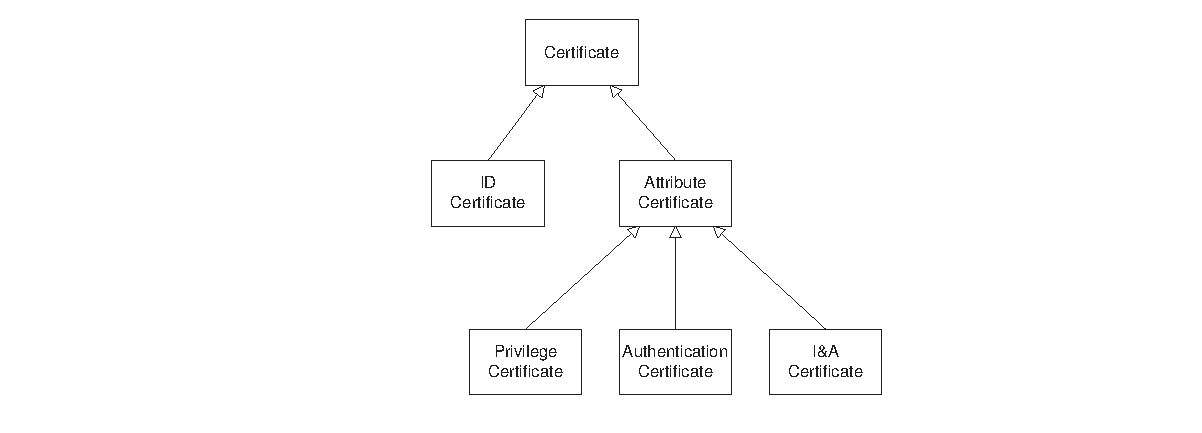
\includegraphics{41_2_certs.eps}}
    \caption{Hierarchy of certificate types}
    \label{fig:certificates}
  \end{center}
\end{figure}

The ID certificate is an X.509 certificate. ID certificates are used
during enrolment as well as being present on tokens.

The subject is the name of the entity being identified by the
certificate and the key is the entity's public key. 

We don't need to know about the key of the Token unless we implement 
the TOKENEER Authentication Protocol or some other secure
comminications protocol between TIS and the Token. Secure
communications with the Token are outside the current scope of this system.

\begin{schema}{IDCert}
	Certificate
\\      subject: USER
\\      subjectPubK: KEYPART
\end{schema}

In general an ID certificate is not validated by the keypart held on
the certificate. 

The ID Certificate of a CA (Certification Authority) is a root
certificate and is signed by itself. The chain of trust has
to start somewhere.

\begin{schema}{CAIdCert}
        IDCert
\where
        isValidatedBy = \{~ subjectPubK ~\} 
\end{schema}


The certificates containing attributes all share some common
attributes. 

All attribute certificates contain the ID of 
the Token and the identification of the ID certificate. Specific types
of attribute certificate build on this common structure.
\begin{schema}{AttCertificate}
        Certificate
\\      baseCertId: CertificateId      
\\      tokenID: TOKENID 
\end{schema}


A privilege certificate additionally contains a role and clearance.
\begin{schema}{PrivCert}
	AttCertificate
\\	role: PRIVILEGE
\\	clearance: Clearance
\end{schema}


An authorisation certificate has the same structure as a privilege certificate.
\begin{schema}{AuthCert}
	AttCertificate
\\	role: PRIVILEGE
\\	clearance: Clearance
\end{schema}

An I\&A (identification and authentication) certificate additionally contains
a fingerprint template. 
\begin{schema}{IandACert}
	AttCertificate
\\	template: FingerprintTemplate
\end{schema}

%..........................
\subsection{Tokens}
%.........................
\label{page:firstTraceunit}
\begin{traceunit}{FS.Types.Tokens}
\traceto{FCO\_NRO.2.1}
\traceto{FCO\_NRO.2.2}
\traceto{FCO\_NRO.2.3}
\traceto{FDP\_DAU.2.1}
\traceto{FDP\_DAU.2.2}
\traceto{FIA\_UAU.3.1}
\traceto{FAI\_UAU.3.2}
\end{traceunit}
\begin{Zcomment}
\item 
Refer to Section \ref{sec:Traceunit} for explanation of the
above tracing block.
\end{Zcomment}
Each Token has a unique ID, ensured unique by the smartcard supplier.
\begin{zed}
	[ TOKENID ]
\end{zed}

A $Token$ contains a number of certificates. The
authorisation certificate is optional while the others must be present.
\begin{schema}{Token}
	tokenID: TOKENID

\also	idCert: IDCert
\\	privCert: PrivCert
\\	iandACert: IandACert
\\	authCert: \Optional AuthCert
\end{schema}


A $Token$ is valid if all of the certificates on it are well-formed,
each certificate correctly cross-references to the ID Certificate,
and each certificate correctly cross-references to the $Token$ ID.

A token need not contain a valid Authorisation certificate to be considered valid.

\begin{schema}{ValidToken}
	Token
\where
	privCert.baseCertId = idCert.id
\\	iandACert.baseCertId = idCert.id

\also	privCert.tokenID = tokenID
\\	iandACert.tokenID = tokenID
\end{schema}

If the Authorisation certificate is present it will only be used if it
is valid, in that it correctly cross-references to the $Token$ ID and
the ID Certificate.

\begin{schema}{TokenWithValidAuth}
	Token
\where
        authCert \neq \Nil 
\\      \t1    \land  (\The authCert).tokenID = tokenID
\\	\t1    \land  (\The authCert).baseCertId = idCert.id
\end{schema}

A $Token$ is current if all of the Certificates are current,
or if only the Auth Cert is non-current.
Currency needs a time, which is included in the schema,
and will need to be tied to the relevent time when this schema is used.

\begin{schema}{CurrentToken}
	ValidToken
\\	now: TIME
\where
	now \in idCert.validityPeriod
\\ \t1		{} \cap privCert.validityPeriod
\\ \t1		{} \cap iandACert.validityPeriod
\end{schema}

%............................
\subsection{Enrolment Data}
%............................

\begin{traceunit}{FS.Types.Enrolment}
\traceto{FMT\_MSA.2.1}
\traceto{FMT\_MTD.3.1}
\end{traceunit}
Enrolment data is the information the ID station needs in order to
know how to authenticate tokens presented to it, and to produce its
own authentication certificates such that they can be authenticated by
workstations in the enclave.

Enrolment data consists of a number of ID certificates: 
\begin{itemize}
\item
this ID Station's ID Certificate, which will be signed by a CA.
\item
A number of other Issuers' ID Certificates. These will belong to 
        \begin{itemize}
        \item
        CAs, who authenticate AAs (Attribute Authorities) and ID Stations. These will be self signed.
        \item
        AAs, who authenticate privilege and I\&A certificates. 
        \end{itemize}
\end{itemize}

The ID Station's certificate is just one of the issuer certificates,
although we will want to be able to identify it as belonging to this
ID station. 

\begin{schema}{Enrol}
        idStationCert : IDCert
\\      issuerCerts : \power IDCert
\where
        idStationCert \in issuerCerts
\end{schema}

For the Enrolment data to be considered valid each certificate must be
signed correctly and the Issuer's certificate must be present for it
to be possible to check that the signatures are correct.
Note that CA ID
certificates are self signed but AA and IDStation certificates are
signed by an CA.

\begin{schema}{ValidEnrol}
        Enrol
\where
        issuerCerts \cap \{ CAIdCert \} \neq \emptyset
\also
\\      \forall cert : issuerCerts @ 
\\      \t1     cert.isValidatedBy \neq \Nil 
\\      \t1     \land (\exists issuerCert : issuerCerts @ 
        issuerCert \in CAIdCert 
\\      \t2     \land \The cert.isValidatedBy = issuerCert.subjectPubK
\\      \t2     \land cert.id.issuer = issuerCert.subject )   
\end{schema}
\begin{Zcomment}
\item
There must be an ID certificate for at least one CA.
\item
For each certificate the enrolment data must include the ID
certificate for the issuer of the certificate, the certificate must be
validated by the issuer's key and the issuer of the
certificate must be a CA.
\end{Zcomment}

%--------------------------------------------------------------------------
\section{World outside the ID Station}
%--------------------------------------------------------------------------
We choose to model the real world (or at least the real peripherals)
as being outside the ID Station.
When the user inserts a token, they are providing input to the ID Station.
It is up to the ID Station to then respond by reading the real world
input into its own, internal representation. The ID Station receives stimulus
from the real world and itself changes the real world. All real world
entities are modelled as components of the $RealWorld$.

We will distingush between real world entities that we use
 (eg. $finger$), we control (eg. $alarm$) 
 and we may change (eg. $userToken$ or $floppy$).


%..............................
\subsection{Real World types}
%..............................

\begin{traceunit}{FS.Types.RealWorld}
\end{traceunit}


There are several types associated with the real world. The door,
latch and alarm all have two possible states.
\begin{zed}
	DOOR ::= open | closed
\also
	LATCH ::= unlocked | locked
\also
	ALARM ::= silent | alarming
\end{zed}

Display messages are the short messages presented to the user on the
small display outside the enclave.
\begin{zed}
	DISPLAYMESSAGE ::= blank | welcome | insertFinger | openDoor |
                        wait | 
\\      \t3  removeToken | tokenUpdateFailed | doorUnlocked
\end{zed}

The messages that appear on the display are presented in table \ref{table:display}.

\begin{table}[h]
\begin{tabular}{|l|l|l|}
                & \multicolumn{2}{c|}{\bf Displayed text} \\ \cline{2-3}
{\bf Message}   & {\bf Top line}                & {\bf Bottom line}     \\
\hline
$blank$         & {\tt SYSTEM NOT OPERATIONAL}  & \\
$welcome$       & {\tt WELCOME TO TIS}          & {\tt ENTER TOKEN}  \\
$insertFinger$  & {\tt AUTHENTICATING USER}     & {\tt INSERT FINGER} \\ 
$wait$          & {\tt AUTHENTICATING USER}     & {\tt PLEASE WAIT} \\
$openDoor$      & {\tt }                        & {\tt REMOVE TOKEN AND ENTER} \\
$removeToken$   & {\tt ENTRY DENIED}            & {\tt REMOVE TOKEN} \\
$tokenUpdateFailed$ &                   & {\tt TOKEN UPDATE FAILED }
\\
$doorUnlocked$  &                       & {\tt ENTER ENCLAVE} \\
\hline
\end{tabular}
\caption{Display Messages}
\label{table:display}
\end{table}

Because it is possible to be trying to read a token that is not inserted,
or a fingerprint when no finger is inserted,
or an invalid token or fingerprint, 
we introduce free types to capture the absence or poor quality of these.

The values $badFP$ and $badT$ represent all possible error codes that
occur when trying to capture this data. The system will behave the
same way in all failure cases with only the audit log capturing the
different error codes that actually occur.
\begin{zed}
	FINGERPRINTTRY ::= noFP | badFP | goodFP \ldata FINGERPRINT \rdata
\also
	TOKENTRY ::= noT | badT | goodT \ldata Token \rdata
\end{zed}

When modelling data supplied on a floppy disk we model the posibility
of the disk not being present, being empty or being corrupt as well as
containing valid data.
We make the assumption that each floppy disk will only contain one
data file, either enrolment data, configuration data or audit data.

\begin{zed}
       FLOPPY ::=  noFloppy | emptyFloppy | badFloppy | 
       enrolmentFile \ldata ValidEnrol \rdata |
\\ \t3    auditFile \ldata \finset Audit \rdata |
          configFile \ldata Config \rdata
\end{zed}

Inputs may be supplied by an administrator at the keyboard. We model
input values representing no data, invalid data or a valid request to
perform an adminstrator operation.

\begin{zed}
        KEYBOARD ::= noKB | badKB | keyedOps \ldata ADMINOP \rdata 
\end{zed}

There are a number of messages that may appear on the TIS screen
within the enclave. Some of these are simple messages, the text of these
is supplied in Table \ref{tab:screen}. 
Others involve more complex presentation of data, such as
configuration data or system statistics, the details of this
presentation is left to design.

\begin{zed}
       SCREENTEXT ::= clear | welcomeAdmin | busy | removeAdminToken |
       closeDoor |
\\ \t3          requestAdminOp | doingOp | invalidRequest | invalidData |
\\ \t3          insertEnrolmentData | validatingEnrolmentData |
       enrolmentFailed |
\\ \t3          archiveFailed | insertBlankFloppy | insertConfigData |
\also 
        \t3  displayStats \ldata Stats \rdata | 
        displayConfigData \ldata Config \rdata
\end{zed}

In addition to the messages statistics and the current configuration
data may be displayed on the screen.

\begin{schema}{Screen}
        screenStats : SCREENTEXT
\\      screenMsg : SCREENTEXT
\\      screenConfig : SCREENTEXT 
\end{schema}

\begin{table}[h]
\begin{tabular}{|l|l|}
{\bf Message}   &  {\bf Displayed text}   \\
\hline
$clear$                 &                               \\
$welcomeAdmin$          & {\tt WELCOME TO TIS}          \\
$busy$                  & {\tt SYSTEM BUSY PLEASE WAIT} \\ 
$removeAdminToken$      & {\tt REMOVE TOKEN} \\
$closeDoor$             & {\tt CLOSE ENCLAVE DOOR} \\
$requestAdminOp$        & {\tt ENTER REQUIRED OPERATION} \\
$doingOp$               & {\tt PERFORMING OPERATION PLEASE WAIT} \\
$invalidRequest$        & {\tt INVALID REQUEST: PLEASE ENTER NEW
OPERATION} \\
$invalidData$           & {\tt INVALID DATA: PLEASE ENTER NEW
OPERATION} \\
$archiveFailed$         & {\tt ARCHIVE FAILED: PLEASE ENTER NEW
OPERATION} \\
$insertEnrolmentData$   & {\tt PLEASE INSERT ENROLMENT DATA FLOPPY} \\
$validatingEnrolmentData$ & {\tt VALIDATING ENROLMENT DATA PLEASE WAIT
} \\
$enrolmentFailed$       & {\tt INVALID ENROLMENT DATA} \\
$insertBlankFloppy$     & {\tt INSERT BLANK FLOPPY} \\
$insertConfigData$      & {\tt INSERT CONFIGURATION DATA FLOPPY} \\
\hline
\end{tabular}
\caption{Short Screen Messages}
\label{tab:screen}
\end{table}

%...............................
\subsection{The Real World}
%...............................

Within this section we consider the entities with which TIS will
interact at an abstract level. We do not consider protocol information
or any flows of information that are not visible to an external
observer. For instance typical fingerprint readers need to have stale
data cleared by TIS to ensure that TIS always reads fresh data. This is
not modelled in this specification but will be introduced during the design.

The real world entities that are controlled by TIS are as follows:
\begin{itemize}
\item the latch on the door into the enclave.
\item the audible alarm.
\item the display that resides outside the enclave.
\item the screen on the ID Station within the enclave with
which the administrator interacts.
\end{itemize}

\begin{schema}{TISControlledRealWorld}
        latch : LATCH
\\      alarm : ALARM
\\      display : DISPLAYMESSAGE
\\      screen : Screen
\end{schema}

The real world entities that are used by TIS are as follows:
\begin{itemize}
\item the real world has a concept of time. This is taken from an
external time source.
\item the door into the enclave that is monitored by the ID Station.
\item fingerprints are read, via the biometric reader, into
the ID Station for comparison with fingerprint templates.
\item a user, trying to enter the enclave will supply
their token to the ID station via the token reader that resides
outside the enclave. 
\item a user within the enclave who has administrator
privileges will supply their token to the ID station via the token
reader that resides inside the enclave.
\item  the ID Station accepts enrolment data and
configuration data on a floppy disk. The disk drive resides in the enclave.
\item  the ID Station has a keyboard within the enclave which the
administrator uses to control TIS. 
\end{itemize}

\begin{schema}{TISMonitoredRealWorld}
        now : TIME
\\      door : DOOR
\\      finger : FINGERPRINTTRY
\\      userToken, adminToken : TOKENTRY
\\      floppy : FLOPPY
\\      keyboard : KEYBOARD
\end{schema}

In addition TIS may change some of the entities that it uses from the
real world.   
\begin{itemize}
\item The ID station may need to update the $userToken$ token
(with an Authentication Certificate).
\item the ID Station archives the Audit Log to floppy disk so may
write to $floppy$.
\end{itemize}

The Whole real world is given by:
\begin{zed}
RealWorld \defs TISControlledRealWorld \land TISMonitoredRealWorld
\end{zed}
